\documentclass[border=10pt]{standalone}
\usepackage[T1]{fontenc}
\usepackage{times}
\usepackage{tikz}
\usetikzlibrary{arrows.meta,positioning}

\begin{document}
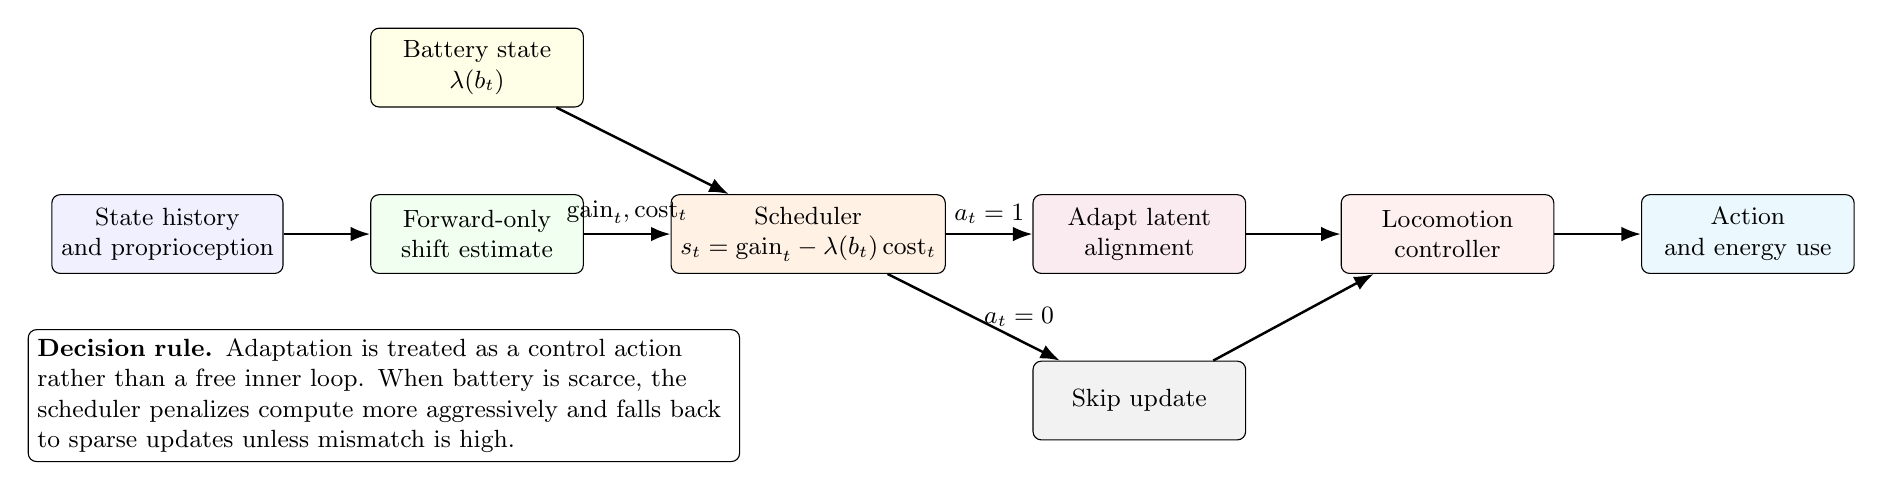
\begin{tikzpicture}[
  >=Latex,
  font=\small,
  box/.style={draw, rounded corners=3pt, align=center, minimum width=2.7cm, minimum height=1.0cm},
  flow/.style={->, line width=0.9pt}
]
\node[box, fill=blue!6] (obs) {State history\\and proprioception};
\node[box, fill=green!6, right=1.1cm of obs] (estimate) {Forward-only\\shift estimate};
\node[box, fill=yellow!10, above=1.1cm of estimate] (battery) {Battery state\\$\lambda(b_t)$};
\node[box, fill=orange!10, right=1.1cm of estimate] (scheduler) {Scheduler\\$s_t = \mathrm{gain}_t - \lambda(b_t)\,\mathrm{cost}_t$};
\node[box, fill=purple!8, right=1.1cm of scheduler] (adapt) {Adapt latent\\alignment};
\node[box, fill=gray!10, below=1.1cm of adapt] (skip) {Skip update};
\node[box, fill=red!6, right=1.2cm of adapt] (controller) {Locomotion\\controller};
\node[box, fill=cyan!8, right=1.1cm of controller] (action) {Action\\and energy use};

\draw[flow] (obs) -- (estimate);
\draw[flow] (estimate) -- node[midway, above] {$\mathrm{gain}_t,\mathrm{cost}_t$} (scheduler);
\draw[flow] (battery) -- (scheduler);
\draw[flow] (scheduler) -- node[midway, above] {$a_t=1$} (adapt);
\draw[flow] (scheduler) -- node[midway, right] {$a_t=0$} (skip);
\draw[flow] (adapt) -- (controller);
\draw[flow] (skip) -- (controller);
\draw[flow] (controller) -- (action);

\node[draw, rounded corners=3pt, align=left, anchor=north west, fill=white, text width=8.8cm] at ([xshift=-0.3cm,yshift=-0.7cm]obs.south west) {%
\textbf{Decision rule.}
Adaptation is treated as a control action rather than a free inner loop.
When battery is scarce, the scheduler penalizes compute more aggressively and falls back to sparse updates unless mismatch is high.};
\end{tikzpicture}
\end{document}
